\chapter{Uplift Modelling}
\label{ch-uplift}



This chapter is based 
on 
many references,
including Ref.\cite{uplift-2017, fei, wiki-uplift,jaros}.

Uphill Modelling (UP)
deals
with  the application of
Rubin's Theory of
Potential Outcomes (PO)
to advertisement and marketing.

PO, which is
discussed in Chapter \ref{ch-pot-out},
 is a subset
of Pearl's Causal Inference.
Besides UP, other  applications of PO theory
that are discussed in this book 
are: Regression Discontinuity (Chapter \ref{ch-reg-dis}),
Difference-in-Differences (Chapter \ref{ch-did})
and Synthetic Controls (Chapter \ref{ch-syn-con}).

In UP,
each {\bf participant person (i.e., sample $\s$)}
is interrogated at two well
anticipated, fairly closely spaced times
$t_0$ and $t_1$ (as opposed to 
Difference-in-Differences  (DID), where
$t_0$ and $t_1$ might
be years apart, and
long before the DID analysis is 
attempted.).
In between those two times,
a treatment which
we will refer to as the
{\bf UP diagnostic test} is applied.
For example,
at times $t_0$ and $t_1$,
every participant
might be asked
how important he/she rates climate 
change on a scale of 1 to 10.
In between times
$t_0$ and $t_1$,
every participant might
be sent a brochure on climate change.

In UP, as in all 
other PO applications, 
each participant
$\s$
is in the 
treated or control
groups, but not both.
The participants
are aware  of which
of those groups they are in,
so they are not \qt{treatment blind}.

\section{UP types}

\begin{figure}[h!]
\centering
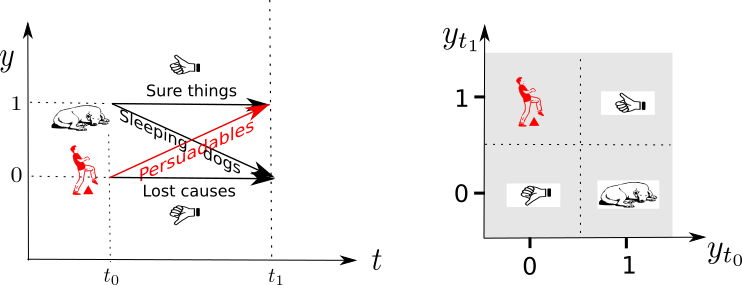
\includegraphics[width=6in]
{uplift/uplift-y-t.png}
\caption{UP diagnostic test
can be used to classify
all participants of the
population into 4 UP-types.
This figure 
assumes $y\in \bool$.
More generally, $y\in \RR$.
$t$ represents time. $t=t_0$
corresponds to $d=0=untreated$,
and $t=t_1$ corresponds to $d=1=treated$.} 
\label{fig-uplift-y-t}
\end{figure}

Let $y^\s_t\in \RR$ for $t=t_0, t_1$
be the treatment response at time $t$
for participant (i.e., sample) $\s$. (We are using here
the same notation as in Chapter \ref{ch-pot-out}).
Call $\delta^\s=
y^\s_{t_1}-y^\s_{t_0}$ the {\bf participant uplift}
for participant $\s$.
As shown
in Fig.\ref{fig-uplift-y-t},
UP classifies participants
into 4 {\bf UP-types}: Persuadables, SureThings, LostCauses,
and SleepyDogs.
The UP-type
of a participant
depends on the changes 
that are induced on that participant
by an {\bf UP-diagnostic-test}.
\begin{itemize}
\item
For a {\bf Persuadable} participant,
$\delta^\s>0$.
\item
For a {\bf SleepyDogs}
participant, $\delta^\s< 0$.
\item
For a {\bf SureThings} participant,
 $\delta^\s\approx 0$
and $y^\s_{t_0}$ is high.
\item
For a {\bf LostCauses} participant,
$\delta^\s\approx 0$
and $y^\s_{t_0}$ is low.
\end{itemize}

In general,
$x=(x_0, x_1,\dots, x_{n-1})$ is an $n$ dimensional 
vector of features $x_i$.
If any of the $x_i$
is a priori continuous, we will
assume it has  been binned into
a finite number of bins.
Let $S_\rvx$ be the finite set of  all feature vectors.


Let $A_x = \{\s: x^\s \approx x\}$ for  $x\in S_\rvx$.
The set $A_x$ of all samples with
a feature vector $x^\s$ close to $x$ 
is called the $x$ {\bf stratum}.



The {\bf stratum-uplift} is
 $\delta_x=ACE_x$.
Strata can also be
classified into
the 4 UP-types,
depending on the sign and size  
of their $\delta_x$.
A participant 
may not be typical for
his stratum
and may
have different
{\bf participant and stratum UP-types}.
For example, he may have positive 
participant uplift $\delta^\s$
and therefore have a Persuadable participant UP-type,
but his stratum-uplift  $\delta_x$
might be negative, so
he has
the SleepyDogs stratum UP-type.

Advertisers are very interested in finding
the Persuadable strata in a population
so as to focus their resources on them.
For example, UP was used very
successfully during the 
Obama presidential campaigns. 
Team Obama conducted UP-diagnostic
tests much like
the climate change one described earlier.
This allowed them to
identify voters who might be sitting on the fence
on whether to vote for Obama or not.
Then Team Obama spent
the lion share
of  resources  on those
fence-sitters.


\section{Some Relevant
 Technical Formulas from Chapter \ref{ch-pot-out}}
Recall
the following technical formulae
that were proven in 
Chapter \ref{ch-pot-out}:

\begin{itemize}

\item
Recall Eq.(\ref{eq-ace-propensity}):

\beq
ACE =\sum_x P(x)
\underbrace{
\sum_y y\left[
P(y|d=1, x)
-
P(y|d=0, x) 
\right]
}_{ACE_x}
\eeq
If $\rvy\in \bool$, then

\beq
\underbrace{ACE_x}_{\displaystyle \delta_x}
=
\underbrace{
P_{\rvy|\rvd, \rvx}(1|1, x)
}_{\displaystyle Y^1_x}
-
\underbrace{
P_{\rvy|\rvd, \rvx}(1|0, x)
}_{\displaystyle Y^0_x}
\;.
\eeq

\item
Recall 
Eq.(\ref{eq-ace-esti-posi}):

\beq
\underbrace{\HAT{ACE_x}}_{\displaystyle\delta_x}
=
\underbrace{
\frac{1}{N_x}
\sum_{\s \in A_x}
\frac{d^\s y^\s}{g_{1|x^\s} }
}_
{\displaystyle Y_x^1}
-
\underbrace{
\frac{1}{N_x}
\sum_{\s \in A_x}
\frac{(1-d^\s)y^\s}{g_{0|x^\s} }
}_
{\displaystyle Y_x^0}
\label{eq-est-ace-uplift}
\eeq




\end{itemize}


\section{UP Analysis}
\label{sec-up-analysis}

The input
to UP is a PO
dataset $DS= \{ (\s, d^\s, x^\s, y^\s):
 \s=0, 1, 2, \ldots, nsam-1\}$.
where $d^\s\in \bool$, $x^\s \in S_\rvx$,
$y^\s\in \RR$.

\begin{figure}[h!]
\centering
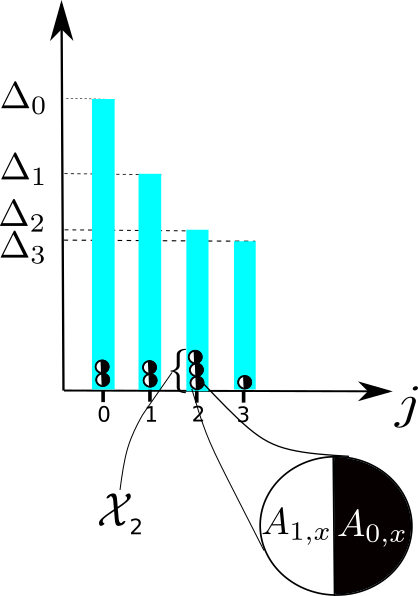
\includegraphics[width=2in]
{uplift/uplift-bins.png}
\caption{
Pictorial
representation
of the sequence
$\{(\calx_c, \Delta_c)\}_{c=0, 1, \ldots, nc-1}$.
}
\label{fig-uplift-bins}
\end{figure}


Starting with $DS$,
UP performs the following steps.
Fig.\ref{fig-uplift-bins}
is a pictorial representation
of the quantities
that are calculated
during these steps.

\begin{enumerate}
\item Find 

\beq
A_x = \{\s: x^\s \approx x\}\eeq
for each observed $x\in S_\rvx$.
Set $A_x=\emptyset$ for unobserved $x\in S_\rvx$.
 
\item Use Eq.(\ref{eq-est-ace-uplift})
to calculate $\delta_x$
for each $x\in S_\rvx$.
Set $\delta_x=0$ if $A_x=\emptyset$.

\item Partition 
the set $\{\delta_x: x\in S_\rvx\}$
into disjoint bins. Call
$\Delta_c$  the average $\delta_x$ 
within bin $c$ for $c=0, 1, \ldots, nc-1$.
The class labels 
$c$ should be assigned
so that the sequence of
$\Delta_c$
is monotonic and non-increasing; i.e.,

\beq
\Delta_0 \geq \Delta_{1}\geq\cdots \geq \Delta_{nc-1}
\;.
\eeq
Now calculate 

\beq
\calx_c =\{ x: \delta_x \approx \Delta_c\}
\eeq
 for each $c$.
By the end of this step,
we will have calculated 
$\{(\calx_c, \Delta_c)\}_{c=0, 1, \ldots, nc-1}$
from $\{(x, \delta_x)\}_{x\in S_\rvx}$.
We will refer to the $\calx_c$
as {\bf strata-bins}. Note that
\beqa
\Delta_c &=&\frac{1}{|\calx_c|}\sum_{x\in\calx_c}\delta_x
\\
&=&
\underbrace{\frac{1}{|\calx_c|}\sum_{x\in\calx_c}Y^1_x}_
{\displaystyle Y^1_c}
- 
\underbrace{\frac{1}{|\calx_c|}\sum_{x\in\calx_c}Y^0_x}_
{\displaystyle Y^0_c}
\;.
\label{eq-Delta-c}
\eeqa
\item
For each $c$,
calculate 

\beq
A_{d,x}=\{\s\in A_x: d^\s = d\}
\eeq

\beq
\Sigma_{d,c}=\cup_{x\in \calx_c}A_{d,x}
\eeq
for $d\in\bool$
and 

\beq
\Sigma_{c}=\Sigma_{0,c}
\cup \Sigma_{1,j}
\;.
\eeq
\end{enumerate}


\begin{figure}[h!]
\centering
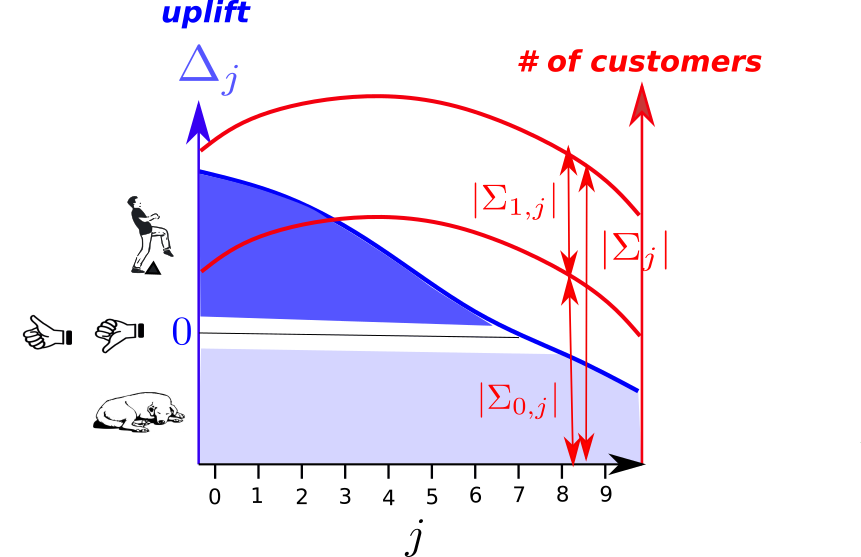
\includegraphics[width=4in]
{uplift/qini-fake.png}

\caption{
Plot
of UP results.
} 
\label{fig-qini-fake}
\end{figure}
Fig.\ref{fig-qini-fake}
is a  way of
plotting
the results 
of UP in an
intuitive
way.


Another common plot of UP results is
called a {\bf Qini
curve}.
A Qini curve is a plot 
of $(X_c,Y_c)$
for all $c$, where

\beq
X_c= \sum_{c'=0}^{c}\sum_{x\in \calx_{c'}}|A_x|
\eeq
is the cumulative population (counting the
samples in
order of decreasing uplift) and

\beq
Y_c=\sum_{c'=0}^c \Delta_{c'}
\eeq
is the cumulative uplift.
As $c$ increases, a Qini curve rises fast at first and then its slope decreases until
at some value $c_0$, the slope is defined as too small to care. No marketing resources are
directed towards
participants $\s$ for whom  $c>c_0$.\footnote{
Let 
$S_{\Delta} = \{\s:\delta^\s \geq \Delta\}$.
A Qini curve can also be defined, without stratification,
as a
 plot of $(X_\Delta, Y_\Delta)$ for all $\Delta>0$,
where $
X_\Delta = |S_{\Delta}|$
and
$
Y_\Delta= \sum_{\s\in S_{\Delta}}\delta^\s
$. As $\Delta$ decreases, a Qini curve rises fast at first and then its slope decreases.
}




\section{UP Decision Trees}

In this section,
we will describe
how to build UP decision trees (UP dtrees),
and explain why they are needed
for UP.

Generic dtrees are 
described in Chapter \ref{ch-dtree}.
This section 
complements rather than replaces
that chapter so the reader
is advised to read
that chapter first.

Ref.\cite{jaros} is an excellent paper on the use of
dtrees in UP.


The
analysis described
previously in  
Section
\ref{sec-up-analysis},
although theoretically correct,
will work very poorly in practice.
The strata-bins
of Section
\ref{sec-up-analysis}
correspond to
the classification
classes of a dtree.
But strata-bins are very
specific so they  
severely overfit the data.
Although dtrees 
can also suffer from overfitting,
there are known methods of 
preventing or mitigating overfitting in dtrees.

There are also tasks 
that dtrees 
can do well
and the methods
explained so far
cannot do well.
For example,
suppose we have 
a classless
dataset $DS^-=\{(\s, x^\s):\s\in \Sigma^-\}$
and we want to predict
the class $c^\s$ and
uplift $\Delta_{c^\s}$
for each of these individuals 
$\s\in \Sigma^-$.
A dtree can easily
do that. The alternative
is to use the classy dataset 
$DS=\{(\s, x^\s, c^\s):\s\in \Sigma\}$
to
prepare a dictionary
that orders
the elements
of $S_\rvx$ and gives a
class $c$ and an uplift value
$\Delta_c$ for each
feature vector $x\in S_\rvx$.
But
such a dictionary overfits
and says nothing for 
feature vectors $x$
that do not show up in 
the classy dataset $DS$; i.e., the
dictionary 
doesn't guess (interpolate). Dtrees,
on the other hand, do
guess.

So, without further ado,
let us describe how to
modify the results
of Chapter \ref{ch-dtree}
on generic dtrees
to the case of UP dtrees.
The main difference,
as we will
explain in detail
next,
is that the Information
Gain metric
used for generic dtrees
needs to be replaced
by another metric.






\begin{figure}[h!]
$$
\xymatrix{
&
\\
\rvx_j\ar[r]_{\rvx_j=x_j}
\ar[ru]^{\rvx_j=x_j'}&
\\
\{N^d_j(c,x_j)\}_{c\in S_\rvc, x_j\in S_{\rvx_j}}
\\
\sum_{c\in S_\rvc}N^d_j(c,x_j)=N^d_j(x_j)
\\
\sum_{x_j\in S_{\rvx_j}}N^d_j(c,x_j)=N^d_j(c)
&
\sum_{c\in S_\rvc}N^d_j(c)=
\sum_{x_j\in S_{\rvx_j}}N^d_j(x_j)=N^d_j
}
$$
\caption{Fig.\ref{fig-dtree-notation}
 with $d$ dependence added.
$d\in \bool$
is the treatment dose.
} 
\label{fig-dtree-notation-uplift}
\end{figure}

\begin{figure}
$$
\xymatrix{
\rvd\ar[dr]\ar[drr]
\\
\rvj
\ar[r]\ar@/^1pc/[rr]
&
\rvx_j\ar[r]
&
\rvc
}$$
\caption{Bnet derived from population
numbers in Fig.\ref{fig-dtree-notation-uplift}}
\label{fig-class-bnet-uplift}
\end{figure}



Fig.\ref{fig-dtree-notation-uplift}
was obtained from Fig.\ref{fig-dtree-notation}
by adding $d$ dependence.
$d\in \bool$
is the treatment dose.
Note that in UP, we build a dtree
in which every node carries a double ($d=0,1$)
TPV. This
is in contrast to the generic dtrees built
in Chapter \ref{ch-dtree}, in which 
each node carries a single TPV.
$N^d_j(c, x_j)$ is 
the number
of individuals $\s$
in the population that reaches node $\rvx_j$
with $d\in \bool$, belonging
to class $c\in S_\rvc$ and having $\rvx_j=x_j$. 
From these population numbers, we can define
the bnet in Fig.\ref{fig-class-bnet-uplift}.
The TPMs, printed in blue,
for the (non-root) nodes of this bnet, are as follows



\beq\color{blue}
P(c|x_j,j,d)=
\frac{N^d_j(c,x_j)}
{N^d_j(x_j)}
\label{eq-p-c-pre-laplace}
\eeq

\beq\color{blue}
P(x_j|j, d)=
\frac{N^d(x_j)}
{N_j^d}
\eeq


In Chapter
\ref{ch-dtree},
we used Information 
Gain
(a mutual information)
as the SAM (Separation Ability Measure)
in
SL (Structure Learning) 
of dtrees (Decision Trees).
Information Gain
is a bad
SAM for SL of UP dtrees,
because it knows nothing about
 $d=0,1$
and the double TPVs of nodes in UP dtrees.
For
UP dtrees,
we need a SAM specifically
designed to separate $d=0,1$, and generate 
classes that are
 uplift bins (i.e., uplift intervals).


Ref.\cite{jaros}
proposes and studies 
the following
3 SAMs 
for doing SL of UP dtrees.


\begin{enumerate}
\item{\bf SAM\_DD} (DD=Delta Delta)

For $d\in \bool$
and $c, c'\in S_\rvc$, define the increments

\beq
\partial_d f(d)=f(1)-f(0)
\eeq
and

\beq
\partial_{c',c} f(c)=f(c')-f(c)
\;.
\eeq
Let

\beqa
\Delta_{c|j} &=& P(c|j,1)-P(c|j,0)
\\
&=& \partial_d P(c|j,d)
\label{eq-delta-c-j}
\eeqa

\beqa
SAM\_DD_j&=& \max_{c,c'}|\partial_{c',c}\partial_d P(c|j,d)|
\\
&=&
\max_{c,c'}|\partial_{c',c}\Delta_{c|j}|
\eeqa

\item{\bf SAM\_KL} (KL=Kullback Leibler)
\begin{align}
SAM\_KL_j&=
\left[
\sum_{x_j\in S_{\rvx_j}}
P(x_j|j)
D_{KL}(P_{\rvc|x_j,j,1}\parallel P_{\rvc|x_j,j,0})
\right]
-
D_{KL}(P_{\rvc|j,1}\parallel P_{\rvc|j,0})
\\
&=
\left[
\sum_{x_j\in S_{\rvx_j}}
P(x_j|j)
 \sum_{c\in S_\rvc}P(c|x_j,j,1) 
\ln \frac{P(c|x_j,j,1) }{ P(c|x_j,j,0) }
\right]
-
\sum_{c\in S_\rvc} 
P(c|j,1) 
\ln \frac{P(c|j,1) }{ P(c|j,0) }
\label{eq-sam-kl}
\end{align}

{\bf $SAM\_KL_j$ can be negative.}

\item {\bf SAM\_E} (E=Euclidean)

$SAM\_E_j$ is defined the same way as $SAM\_KL_j$
except with 
the KL divergence $D_{KL}(P\parallel Q)$ 
in $SAM\_KL$ replaced 
by the Euclidean distance squared. 


\beq
D(P,Q) =\sum_x (P(x)-Q(x))^2
\eeq

\end{enumerate}

The intuitive reason for
 using these quantities as
SAMs is that they maximize the change in uplift 
between 
successive tree levels, so 
that the uplift increases as quickly as possible
as we descend down the UP tree.
In the case of generic dtrees
for which we use Information Gain as SAM, we 
are maximizing the correlation
between classes and nodes as we descend down the tree. 
These two goals are related.
In fact, in the limit
where the
number of control individuals
becomes zero,
$SAM\_KL_j$ and $IG_j$
become the same, as will be shown later.

Next we show
that $SAM\_KL_j$
satisfies the following 3
axioms\footnote{
We won't show it
here, but 
according to Ref.\cite{jaros},
$SAM\_E_j$ also satisfies these
3 axioms, but
$SAM\_DD_j$
satisfies only the first two.}

\begin{claim}
.\newline
\begin{enumerate}
\item \label{item-sam-min}
$SAM\_KL_j$ 
is minimum
iff 
$P(c|x_j,j,0)=P(c|x_j, j,1)$ 
for all $c$ and $x_j$.
\item \label{item-sam-zero}
If $P(c|j,d)=P(c|d)$
for all $c,d$, then $SAM\_KL_j=0$.
\item
\label{item-no-control}
Suppose $N^0_r=0$ for all nodes $r\in J_0$
 (i.e., no control population)
and we use the Laplace Correction
when warranted. Then

\begin{align}
SAM\_KL_j
&=
H(\rvc:\rvx_j|j,1)
\\
&=
IG_j\;\;\; \text{ for treated population}
\;.
\end{align}
\end{enumerate}
\end{claim}
\proof

The proof of items
\ref{item-sam-min}
and \ref{item-sam-zero}
follow by inspection of Eq.(\ref{eq-sam-kl}).
Item \ref{item-no-control}
is proven in Claim \ref{claim-no-control}
below.
\qed



Let $N_\rvc=|S_\rvc|$.
Define the uniform probability 
distribution 

\beq
U_\rvc(c)=\frac{1}{N_\rvc}
\eeq
for all $c\in S_\rvc$.

Eq.(\ref{eq-p-c-pre-laplace})
for the TPM of node
$\rvc$ in the bnet Fig.\ref{fig-class-bnet-uplift} can be
\qt{Laplace Corrected}
as follows
so that it is no longer
undefined when
its denominator vanishes:

\beq
P(c|j,d)=
\left\{
\begin{array}{ll}
\frac{N^d_j(c)}
{N^d_j}&\text{ if } N^d_j>0
\\
U_\rvc(c) & \text{ if $N^d_j=0$ (Laplace Correction)}
\end{array}
\right.
\eeq




\begin{claim}
\label{claim-no-control}
Suppose $N^0_r=0$ for all dtree nodes $r\in J_0$
and we use the Laplace Correction
when warranted. Then

\beq
SAM\_KL_j=H(\rvc:\rvx_j|j,1)
\;.
\eeq
\end{claim}
\proof

For all nodes $r\in J_0$, we  must have

\beq
P_{\rvc|r,0}=U_\rvc
\eeq
so

\beqa
D_{KL}(P_{\rvc|r,1}\parallel P_{\rvc|r,0})
&=&
D_{KL}(P_{\rvc|r,1}\parallel U_\rvc)
\\
&=&
\ln(N_\rvc) - H(\rvc|r,1)
\;.
\label{eq-kl-reduce}
\eeqa
For all $x_j\in S_{\rvx_j}$, we must also have


\beq
N_j=N_j^1,  N(x_j)=N^1(x_j)
\eeq
so

\beq
P(x_j|j)=
P(x_j|j,1)
\;.
\label{eq-p-kj-add-1}
\eeq
Now using Eqs.(\ref{eq-kl-reduce}) and
 (\ref{eq-p-kj-add-1}), we get


\beqa
SAM\_KL_j&=&
-\left[
\sum_{x_j\in S_{\rvx_j}}
P(x_j|j)
H(\rvc|x_j,j,1)
\right]
+
H(\rvc|j,1)
\\
&=&
-\left[
\sum_{x_j\in S_{\rvx_j}}
P(x_j|j,1)
H(\rvc|x_j,j,1)
\right]
+
H(\rvc|j,1)
\\
&=&
-H(\rvc|\rvx_j,j,1)+H(\rvc|j,1)
\\
&=&
H(\rvc:\rvx_j|j,1)
\eeqa
\qed


\subsection{Appendix, 
connection between
$\Delta_c$
and $\Delta_{c|j}$}

Recall Eq.(\ref{eq-Delta-c}):

\beqa
\Delta_c &=& 
\underbrace{\frac{1}{|\calx_c|}\sum_{x\in\calx_c}Y^1_x}_
{\displaystyle Y^1_c}
- 
\underbrace{\frac{1}{|\calx_c|}\sum_{x\in\calx_c}Y^0_x}_
{\displaystyle Y^0_c}
\\
&=&
\partial_d Y^d_c
\;.
\eeqa
Compare that to Eq.(\ref{eq-delta-c-j}):
\beqa
\Delta_{c|j} &=& P(c|j,1)-P(c|j,0)
\\
&=& \partial_d P(c|j,d)
\eeqa
What is the connection
between these 2 deltas, $\Delta_c$
and $\Delta_{c|j}$? Are they equal?

First off, notice that 
$\Delta_{c|j}$ is defined for all 
nodes $j$ of the dtree. Let 
$j(c)$ be the leaf node 
for which $\Delta_c\approx \Delta_{c|j(c)}$. 
Assume $y^\s\in\bool$. Then

\beq
P(c|j=j(c), d)=\frac{N^d_{j(c)}(c)}{N^d_{j(c)}}
\approx Y^d_c
\eeq
So the two deltas are indeed approximately equal
when $y^\s\in \bool$ and $j=j(c)$.

